\documentclass{article}
\usepackage{amssymb,amsmath,blindtext,listings,graphicx}
\title{Linear Least Squares Line Fitting Calculus}
\date{2025 March}
\author{Sean Brennan \\ www.zettix.com \\ github.com/zettix}
\begin{document}
\maketitle


\section{Introduction}
This is a description of fitting a line to a collection of
two dimensional points $(x,y)$ by minimizing the error defined
as the square of the differences between the line $y = mx + b$ and each $y_i$ for every $x_i$ in the point set, when added together.  Below is an example of
a solution of the best fitting line given the illustrated points.

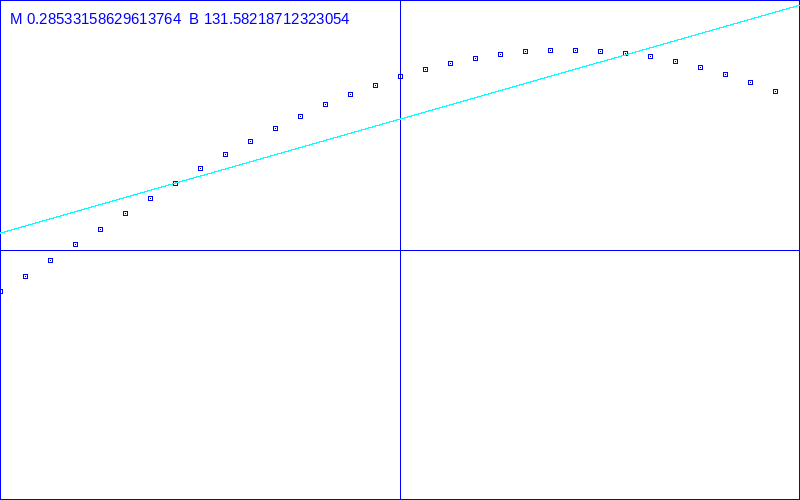
\includegraphics[width=110mm]{whiteplot.png}

To find the line, we define our error function. Described below,
it is sometimes called the sum of residuals. The important idea is that
it is a function, and thus has parameters and a derivative.

To find the minimum, we take the derivative, or gradient, and set it to zero.
This is possible because the function $z = (x - y)^2$ is convex and increases
as $x$ and $y$ differ, the minimum value has gradient zero.  This is like
our error function which is a sum of squares.

\section{The error function}

The error function is defined as the differences between
the line's $y$ values and the $y$ values of the data set squared for each pair.
\begin{equation}
\sum_{i=1}^{n}\left(m x_i + b - y_i\right)^2
\end{equation}

We can see this as a function $f$ taking two variables, $m$ and $b$:
\begin{equation}
f(m, b) = \sum_{i=1}^{n}\left(m x_i + b - y_i\right)^2
\end{equation}


\section{Finding the minimum: Simplfy}

The current definition of $f(m, b)$ would require the chain rule for a
derivative, in a sum, things we can avoid by trying to isolate our terms
by carrying out the square, isolating the sums from our parameters ${\bf m}$
and ${\bf b}$ and separating constants from our variables.

Dropping the sum for the moment, we expand:
\begin{equation}
\begin{split}
f(m, b) & = \left(m x_i + b - y_i\right)^2\\
 & = \left(m x_i + b - y_i\right)\left(m x_i + b - y_i\right)\\
 & = m x_i \left(m x_i + b - y_i\right) + b \left(m x_i + b - y_i\right) - y_i \left(m x_i + b - y_i\right) \\
 & = m x_i m x_i + m x_i b - m x_i y_i + b m x_i + b^2 - b y_i - y_i m x_i - y_i b + y_i^2 \\
 & = m^2 x_i^2 + m b x_i  - m x_i y_i + m b x_i + b^2 - b y_i - m y_i x_i - b y_i + y_i^2 \\
 & = m^2 x_i^2 + 2 m b x_i  - 2 m x_i y_i - 2 b y_i + b^2 + y_i^2 
\end{split}
\end{equation}
If we add the sum back we get:
\begin{equation}
f(m, b) = \sum_{i=1}^n \left( m^2 x_i^2 + 2 m b x_i  - 2 m x_i y_i - 2 b y_i + b^2 + y_i^2 \right)
\end{equation}
Expanding the sums, carefully:
\begin{equation}
f(m, b) = \sum_{i=1}^n m^2 x_i^2 + \sum_{i=1}^n 2 m b x_i  - \sum_{i=1}^n 2 m x_i y_i - \sum_{i=1}^n 2 b y_i + \sum_{i=1}^n b^2 + \sum_{i=1}^n y_i^2 
\end{equation}
Then factoring and simplifying:
\begin{equation}
f(m, b) = m^2 \sum_{i=1}^n x_i^2 + 2 m b \sum_{i=1}^n  x_i  - 2 m \sum_{i=1}^n x_i y_i - 2 b \sum_{i=1}^n y_i + n b^2 + \sum_{i=1}^n y_i^2 
\end{equation}

\section{Summed Constants}

We know the sums of $x_i$ and $x_i^2$ are constant, that is, we cannot change them, we using them to define our gradient.
So let's rename them to simplify our calculations.
\begin{equation}
\chi = \sum_{i=1}^n x_i
\end{equation}
And
\begin{equation}
\Omega = \sum_{i=1}^n x_i^2
\end{equation}
With
\begin{equation}
\upsilon = \sum_{i=1}^n y_i
\end{equation}
And finally
\begin{equation}
\phi = \sum_{i=1}^n x_i y_i
\end{equation}

The equation above becomes more simple:
\begin{equation}
f(m, b) = m^2 \Omega + 2 m b \chi - 2 m \phi - 2 b \nu + n b^2 + \sum_{i=1}^n y_i^2 
\end{equation}

The final sum does not involve our parameters $m$ or $b$ so we don't simplify it, we will ignore it.

\section{Finding the minimum: derivatives of  $f(m, b)$}
Now let's get the gradient by taking partial derivatives using our two knobs: $m$ and $b$:
Let us first solve for $m$.
\begin{equation}
\frac{\partial f(m,b)}{\partial m} = 2 m \Omega + 2 b \chi  - 2 \phi
\end{equation}
Then, by $b$
\begin{equation}
\frac{\partial f(m,b)}{\partial b} = 2 m \chi - 2 \nu + 2 n b
\end{equation}
Setting both to zero, and dividing by two, we get:
\begin{equation}
\label{dm}
\frac{\partial f(m,b)}{\partial m} = m \Omega + b \chi - \phi = 0
\end{equation}
And
\begin{equation}
\label{db}
\frac{\partial f(m,b)}{\partial b} =  m \chi + nb - \nu = 0
\end{equation}
Find a common factor for ${\bf b}$ by multiplying \eqref{dm} by ${\bf n}$ and \eqref{db} by ${\bf -\chi}$
\begin{equation}
m {\bf n}  \Omega +  b \chi {\bf n}  -  \phi {\bf n} = 0
\end{equation}
And
\begin{equation}
- m {\bf \chi^2}  - b {\bf \chi} n  +  \upsilon {\bf \chi} = 0
\end{equation}
Adding them and removing the $-b\chi n$ term.
\begin{equation}
{\bf m} \left( n \Omega - \chi^2 \right) + \upsilon \chi - \phi n = 0
\end{equation}
Move $\nu \chi$ and $\phi n$ to the other side, and divide by
$n \Omega - \chi^2$ and we get the first half of our solution, ${m}$
\begin{equation}
{\bf m} = \frac{\phi n - \upsilon \chi }{n \Omega - \chi^2}
\end{equation}

Should we divide by zero, the slope will become $\infty$!
We deal with that in the next section.
Should $n \Omega - \chi^2$ not be zero, we can find $b$ with:
\begin{equation}
{\bf b} \chi = \phi - m \Omega 
\end{equation}
Finally:
\begin{equation}
{\bf b} = \frac{\phi - m \Omega}{\chi}
\end{equation}

\section{Corner cases}

Notice the two pitfalls:  $\chi = 0$ and $n \Omega - \chi^2 = 0$!   What
do these mean?   $\chi = 0$ implies:
\begin{equation}
\sum_{i=1}^n x_i = 0
\end{equation}
This is not difficult.  Consider the points: $(-1, 1), (0, 2), (1, 3)$.
Starting at $(-1, 1)$, the line has slope 1 and $y$ intercept of 2.
Nevertheless, the sum of ${\bf x_i}$ is zero i.e. ${\chi}$ is zero and the
equation for ${\bf b}$ fails.

Hence we try an alternate strategy: solve for ${\bf b}$ instead of ${\bf m}$.
Find a common factor for ${\bf m}$ by multiplying \eqref{dm} by ${\bf \chi}$
 and \eqref{db} by ${\bf -\Omega}$

\begin{equation}
 m \Omega \chi + b \chi^2 - \phi \chi = 0
\end{equation}

\begin{equation}
- m \chi \Omega - n b \Omega + \nu \Omega = 0
\end{equation}

Add them up, and we get:
\begin{equation}
 b \chi^2 - n b \Omega + \nu \Omega - \phi \chi  = 0
\end{equation}

Collecting ${\bf b}$ and moving constants to the other side:
\begin{equation}
b (\chi^2 - n \Omega) =  \phi \chi - \nu \Omega
\end{equation}

We are in a contingency, where $\chi = 0$, so let us exploit this to simplify.
\begin{equation}
n \Omega b =  \nu \Omega
\end{equation}

Immediately:
\begin{equation}
b = \frac{\nu \Omega}{n \Omega} = \frac{\nu}{n}
\end{equation}

Things get even more weird using \eqref{db} with $\chi = 0$ to find ${\bf m}$:
\begin{equation}
m \Omega - \phi = 0
\end{equation}

And hence:
\begin{equation}
m = \frac{\phi}{\Omega}
\end{equation}

Now to deal with pitfall two: $n \Omega - \chi^2 = 0$, or:
\begin{equation}
n  \left( \sum_{i=1}^n x_i^2 \right) - \left( \sum_{i=1}^n x_i \right)^2 = 0
\end{equation}

For example, a single point will create that problem, and a single point
has no solution, nor does a set where all the $x$ values are identical. Here is what we want to avoid:
\begin{equation}
n  \left( \sum_{i=1}^n x_i^2 \right) = \left( \sum_{i=1}^n x_i \right)^2
\end{equation}

If $\mid{\bf \vec{x} }\mid > 0$ then we cannot have the two sums equal due to
the  Cauchy–Schwarz Inequality:

\begin{equation}
\mid\left<{\bf u},{\bf v}\right>\mid^2 \
\le \left<{\bf u},{\bf u}\right>\cdot\left<{\bf v},{\bf v}\right>
\end{equation} 
where ${\bf u}$ is $\vec{x}$ and ${\bf v}$ is $[1, 1, 1, ..., 1]$, and
$< , >$ is the inner (dot) product, while the actual dot($\cdot$) is a
scalar multiply.   Hence we see that $<{\bf v}, {\bf v}> = n$, and the others
match the above equation as well.

So if we get an equality, we simply report an error.

\vfill

\section{Code}
A function to obtain ${\bf m}$ and ${\bf b}$ is given below, as you can see,
it is quite short.
\lstset{language=Python}
\begin{lstlisting}[frame=single]
def FindLine(points=[]):
    """points is a 2-D array
        [[x, y], [x, y], ...]"""
    chi = 0.0
    omega = 0.0
    nu = 0.0
    phi = 0.0

    n = len(points)
    for x, y in points:
      chi += x
      omega += x * x
      nu += y
      phi += x * y

    if chi == 0.0:  # special case.
      m = phi / omega
      b = nu / n
      return (m, b)

    d = n * omega - chi * chi
    if d == 0.0:
      raise Exception("Bad data!")
    m = (chi + phi * n - nu * chi) / d
    b = (phi - m * omega) / chi
    return (m, b)
\end{lstlisting}

\section{Conclusion}

By using partial derivatives and some algebra, it is fairly easy to
understand how to fit a line to a collection of points.  This is
called Gradient Descent and is used in Inverse Kinematics and
Artificial Intelligence.

\end{document}
